\documentclass[11pt]{article}

\usepackage{amsthm,amsfonts,amsmath,algonjk}
\usepackage{graphicx,url,xspace}
\usepackage{picins,pifont,boxedminipage}
\usepackage{tikz}
\usepackage{hyperref}

\def\Comment#1{\textsl{#1\/}}


\textheight 9.1in
\advance \topmargin by -1.0in
\textwidth 6.7in
\advance \oddsidemargin by -0.8in
\newcommand{\myparskip}{3pt}
\parskip \myparskip

\setcounter{tocdepth}{2}
\newcounter{thm0Rcopies}
\newcounter{thm_saved}

\newtheorem{fact}{Fact}[section]
\newtheorem{lemma}{Lemma}[section]
\newtheorem{theorem}[lemma]{Theorem}
\newtheorem{assumption}[lemma]{Assumption}
\newtheorem{definition}[lemma]{Definition}
\newtheorem{corollary}[lemma]{Corollary}
\newtheorem{prop}[lemma]{Proposition}
\newtheorem{claim}[lemma]{Claim}
\newtheorem{remark}[lemma]{Remark}
\newtheorem{prob}{Problem}
\newtheorem{conjecture}{Conjecture}
\newcommand{\yes}{{\sc Yes-Instance}\xspace}
\newcommand{\no}{{\sc No-Instance}\xspace}

\newenvironment{note}[1]{\medskip\noindent \textbf{#1:}}{\medskip}


\newcommand{\opt}{\textsc{OPT}}
\newcommand{\etal}{{\em et al.}\ }
\newcommand{\ignore}[1]{}
\newcommand{\mc}[2]{\multicolumn{#1}{c}{#2}}

\def\pt{\script{P}_t}
\def\eps{\varepsilon}
\def\bar{\overline}
\def\floor#1{\lfloor {#1} \rfloor}
\def\ceil#1{\lceil {#1} \rceil}
\def\script#1{\mathcal{#1}}
\def\prof#1{\textrm{profit}(#1)}
\def\stdLP{\eqref{eq:std}\xspace}
\def\KCLP{\eqref{eq:kc}\xspace}
\def\kway{-Way---Connected Subgraph\xspace}
\def\P{\script{P}}
\def\C{\script{C}}
\def\dmax{d_{\max}}
\def\dmin{d_{\min}}
\def\ni{\noindent}
\def\RG{{\sc Reverse-Greedy}\xspace}
\def\leader{\texttt{Leader}}
\def\hleader{h\texttt{-Leader}}
\def\class{{\tt class}} 
\def\capR{Cap--Connected Subgraph\xspace}

\renewenvironment{proof}{\vspace{-0.1in}\noindent{\bf Proof:}}{\hspace*{\fill}\par}
\newenvironment{proofof}[1]{\smallskip\noindent{\bf Proof of #1:}}{\hspace*{\fill}\par}
\newenvironment{proofsketch}{\vspace{-0.1in}\noindent{\bf Proof Sketch:}}{\hspace*{\fill}\par}

\title{Approximability of Capacitated Network Design}
\author{
Deeparnab Chakrabarty\thanks{Department of Computer and Information Science, University of Pennsylvania,
Philadelphia PA. Email: {\tt deepc@seas.upenn.edu}.}
\and
Chandra Chekuri\thanks{Dept. of Computer Science, University of Illinois,
Urbana, IL 61801. Partially supported by NSF grants CCF-0728782 and
CNS-0721899. {\tt chekuri@cs.illinois.edu}}
\and
Sanjeev Khanna \thanks{Dept. of Computer \& Information Science, University of Pennsylvania,
Philadelphia, PA 19104. Supported in
part by NSF Awards CCF-0635084 and IIS-0904314. {\tt sanjeev@cis.upenn.edu}}
\and
Nitish Korula\thanks{Dept. of Computer Science, University of Illinois, Urbana,
    IL 61801. Partially supported by NSF grant CCF 0728782 and a
    University of Illinois Dissertation Completion Fellowship. {\tt
      nkorula2@illinois.edu}}
}
\date{}
\begin{document}
\maketitle
\begin{abstract}
  In the {\em capacitated} survivable network design problem
  (Cap-SNDP), we are given an undirected multi-graph where each edge
  has a capacity and a cost.  The goal is to find a minimum cost
  subset of edges that satisfies a given set of pairwise minimum-cut
  requirements.  Unlike its classical special case of SNDP when all
  capacities are unit, the approximability of Cap-SNDP is not well
  understood; even in very restricted settings no known algorithm
  achieves a  approximation, where  is the number of edges in
  the graph. In this paper, we obtain several new results and insights
  into the approximability of Cap-SNDP.

  We give an  approximation for a special case of Cap-SNDP
  where the global minimum cut is required to be at least . (Note
  that this problem generalizes the min-cost -edge-connected
  subgraph problem, which is the special case of our problem when all
  capacities are unit.)  Our result is based on a rounding of a
  natural cut-based LP relaxation strengthened with knapsack-cover
  (KC) inequalities. Our technique extends to give a similar
  approximation for a new network design problem that captures global
  minimum cut as a special case.  We then show that as we move away
  from global connectivity, even for the single pair case (that is,
  when only one pair  has positive connectivity requirement),
  this strengthened LP has  integrality gap.  Furthermore,
  in directed graphs, we show that single pair Cap-SNDP is
  -hard to approximate for any fixed
  constant .

  We also consider a variant of the Cap-SNDP in which multiple copies
  of an edge can be bought: we give an  approximation for
  this case, where  is the number of vertex pairs with non-zero
  connectivity requirement. This improves upon the previously known
  -approximation for this problem when the
  largest minimum-cut requirement, namely , is large. On the
  other hand, we observe that the multiple copy version of Cap-SNDP is
  -hard to approximate even for the single-source
  version of the problem.
\end{abstract}
\thispagestyle{empty}
\newpage
\setcounter{page}{1}
\section{Introduction}
In this paper we consider the {\em capacitated} survivable network
design problem (Cap-SNDP). The input consists of an undirected
-vertex multi-graph  and an integer requirement 
for each unordered pair of nodes . Each edge  of  has a
cost  and an integer capacity . The goal is to find a
minimum-cost subgraph  of  such that for each pair of nodes
 the capacity of the minimum-cut between  and  in  is at
least . This generalizes the well-known survivable network
design problem (SNDP) problem in which all edge capacities are
. SNDP already captures as special cases a variety of fundamental
connectivity problems in combinatorial optimization such as the
min-cost spanning tree, min-cost Steiner tree and forest, as well as
min-cost -edge-connected subgraph; each of these problems has been
extensively studied on its own and several of these special cases are
NP-hard and APX-hard to approximate. Jain, in an influential paper
\cite{Jain}, obtained a -approximation for SNDP via the standard
cut-based LP relaxation using the iterated rounding technique.

Although the above mentioned -approximation for SNDP has been known
since 1998, the approximability of Cap-SNDP has essentially been wide
open even in very restricted special cases.  Similar to SNDP, Cap-SNDP
is motivated by both practial and theoretical considerations. These
problems find applications in the design of resilient networks such as
in telecommunication infrastructure. In such networks it is often
quite common to have equipment with different discrete capacities;
this leads naturally to design problems such as Cap-SNDP.  At the
outset, we mention that a different and somewhat related problem is
also referred to by the same name, especially in the operations
research literature. In this version the subgraph  has to support
{\em simultaneously} a flow of  between each pair of nodes
; this is more closely related to multicommodity flows and
buy-at-bulk network design. Our version is more related to
connectivity problems such as SNDP.

As far as we are aware, the version of Cap-SNDP that we study was
introduced (in the approximation algorithms literature) by Goemans
\etal \cite{GG+} in conjunction with their work on SNDP. They made
several observations on Cap-SNDP: (i) Cap-SNDP reduces to SNDP if all
capacities are the same, (ii) there is an 
approximation where  is the number of edges in  and  is the maximum requirement, and (iii) if {\em
  multiple} copies of an edge are allowed then there is an -approximation.  We note that in the capacitated case
 can be exponentially large in , the number of nodes of
the graph. Carr \etal \cite{CFLP} observed that the natural cut-based
LP relaxation has an unbounded integrality gap even for the graph
consisting of only two nodes  connected by parallel edges with
different capacities. Motivated by this observation and the goal of
obtaining improved approximation ratios for Cap-SNDP, \cite{CFLP}
strengthened the basic cut-based LP by using {\em knapsack-cover}
inequalities. (Several subsequent papers in approximation algorithms
have fruitfully used these inequalities.) Using these inequalities,
\cite{CFLP} obtained a  approximation for Cap-SNDP where
 is the maximum cardinality of a \emph{bond} in the
underlying simple graph: a bond is a minimal set of edges that
separates some pair of vertices with positive demand. Although
 could be  in general, for certain topologies
--- for instance, if the underlying graph is a line or a cycle ---
this gives constant factor approximations.

The above results naturally lead to several questions.  What is the
approximability of Cap-SNDP? Should we expect a poly-logarithmic
approximation or even a constant factor approximation?  If not, what
are interesting and useful special cases to consider?  And do the
knapsack cover inequalities help in the general case?  What is the
approximability of Cap-SNDP if one allows multiple copies? Does this
relaxed version of the problem allow a constant factor
approximation?

In this paper we obtain several new positive and negative results for 
Cap-SNDP that provide new insights into the questions above.

\iffalse

In this paper, we also study the so called {\em soft capacity} version
of Cap-SNDP.  In this version, each edge  can be bought any number
of times; that is, one can pay cost  to get a capacity of
, for any positive integer . Such a variant is natural
in some application settings; for example, one may be able to
simultaneously lay down multiple copies of a telecommunications cable
across two nodes.  We will sometimes call the original version of the
problem one with {\em hard} capacities, when we want to make a
distinction between the two versions.
\fi


\subsection{Our Results}
We first discuss results for Cap-SNDP where multiple copies are not
allowed.  We initiate our study by considering the {\em global
  connectivity} version of Cap-SNDP where we want a min-cost subgraph
with global min-cut at least ; in other words, there is a
``uniform'' requirement  for {\em all} pairs . We
refer to this as the {\em \capR} problem; the special case when all
capacities are unit corresponds to the classical minimum cost
-edge-connected (spanning) subgraph problem, which is known to be APX-hard \cite{Fer}.  We show the following positive
result for arbitrary capacities.

\begin{theorem}\label{thm:uniform}
  There is a randomized -approximation algorithm for the
  \capR problem.  Moreover, for any , there is a
  randomized -approximation algorithm with running
  time  for ``nearly uniform'' Cap-SNDP when all
  pairwise requirements are in .
\end{theorem}

To prove Theorem \ref{thm:uniform}, we begin with a natural LP
relaxation for the problem. Almost all positive results previously
obtained for the unit capacity case are based on this relaxation. As
remarked already, this LP has an unbounded integrality gap even for a
graph with two nodes (and hence for \capR). We strengthen the
relaxation by adding the valid knapsack cover inequalities.  Although
we do not know of a polynomial time algorithm to separate over these
inequalities, following \cite{CFLP}, we find a violated inequality
{\em only if} the current fractional solution does not satisfy certain
useful properties. Our main technical tool both for finding a violated
inequality and subsequently rounding the fractional solution is
Karger's theorem on the number of small cuts in undirected graphs
\cite{Karger}.

We believe the approach outlined above may be useful in other network
design applications. As a concrete illustration, we use it to solve an
interesting and natural generalization of \capR, namely, the {\em
  \kway} problem.  The input consists of  integer requirements
, such that . The goal is to find a minimum-cost subgraph  of  such
that for each , the capacity of any -way cut
of  is at least .\footnote{An -way cut  of a graph
   is a partition of its vertices into  non-empty sets
  ; we use  to denote the set of edges
  with endpoints in different sets of the partition .  The
  \emph{capacity} of an -way cut  is the total capacity of
  edges in .} It is easy to see that \capR is precisely
the \kway, with .  Note that the \kway problem is not a special
case of the general Cap-SNDP as the cut requirements for the former
problem are not expressible as pairwise connectivity constraints.
Interestingly, our techniques for \capR can be naturally extended to
handle the multiway cut requirements, yielding the following
generalization of Theorem~\ref{thm:uniform}.

\begin{theorem}\label{thm:kWay}
  There is a randomized -approximation algorithm for the
  \kway problem with  running time.
\end{theorem}

We remark that even for the unit-capacity case of this problem, it is
not clear how to obtain a better ratio than that guaranteed by the
above theorem. We discuss more in Section~\ref{subsec:kway}.

Once the pairwise connectivity requirements are allowed to vary
arbitrarily, the Cap-SNDP problem seems to become distinctly harder.
Surprisingly, the difficulty of the general case starts to manifest
even for the simplest representative problem in this setting, where
there is only one pair  with ; we refer to this as
the {\em single pair} problem.  The only known positive result for
this seemingly restricted case is a polynomial-factor approximation
that follows from the results in \cite{GG+,CFLP} for general Cap-SNDP.
We give several negative results to suggest that this special case may
capture the essential difficulty of Cap-SNDP.  In particular, we start
by observing that the LP with knapsack cover inequalities has an
 integrality gap even for the single-pair
problem.\footnote{In \cite{CFLP} it is mentioned that there is a
  series-parallel graph instance of Cap-SNDP such that the LP with
  knapsack-cover inequalities has an integrality gap of at least
  . However, no example is given; it is not
  clear if the gap applied to a single pair instance or if 
  could be as large as  in the construction.} Next we show that
the single pair problem is -hard to approximate.
  

\begin{theorem}\label{thm:singlePairHardness}
  The single pair Cap-SNDP problem cannot be approximated to a factor
  better than  unless .
\end{theorem}

The above theorem is a corollary of the results in Chuzhoy \etal's
work on the hardness of related network design problems
\cite{CGNS}. We state it as a theorem to highlight the status of the
problem. (See Appendix~\ref{app:copiesHardness} for a brief proof
sketch.)  We further discuss this connection at the end of this
section. We prove a much stronger negative result for the single pair
problem in {\em directed} graphs. Since in the unit-capacity case,
polynomial-time minimum-cost flow algorithms solve the single-pair
problem exactly even in directed graphs, the hardness result below
shows a stark contrast between the unit-capacity and the non-unit
capacity cases.

\begin{theorem}\label{thm:stHardness}
  In {\em directed} graphs, the single pair Cap-SNDP cannot be approximated to a
  factor better than  for any ,
  unless . Moreover, this hardness
  holds for instances in which there are only two distinct edge capacities.
\end{theorem}


\paragraph{Allowing Multiple Copies:} Given the negative results above
for even the special case of the single-pair Cap-SNDP, it is natural
to consider the relaxed version of the problem where multiple copies
of an edge can be chosen. Specifically, for any integer ,
 copies of  can be bought at a cost of  to
obtain a capacity .  In some applications, such as in
telecommunication networks, this is a reasonable model. As we
discussed, this model was considered by Goemans \etal \cite{GG+} who
gave an  approximation for Cap-SNDP. This follows
from a simple  approximation for the case when all requirements
are in .  The advantage of allowing multiple copies is that
one can group request pairs into classes and separately solve the
problem for each class while losing only the number of classes in the
approximation ratio.  For instance, one easily obtains a
-approximation for the single pair problem even in directed graphs,
in contrast to the difficulty of the problem when multiple copies are
not allowed. Note that this also implies an easy  approximation
where  is the number of pairs with . We address the
approximability of Cap-SNDP with multiple copies of edges allowed.
When  is large, we improve the -approximation discussed above via the following.

\begin{theorem}\label{thm:multipleCopies}
  In undirected graphs, there is an -approximation
  algorithm for Cap-SNDP with multiple copies, where  is the number
  of pairs with .
\end{theorem}

Both our algorithm and analysis are inspired by the
-competitive online algorithm for the Steiner forest
problem by Berman and Coulston~\cite{BC}, and the subsequent
adaptation of these ideas for the priority Steiner forest problem by
Charikar \etal \cite{CNS}. However, we believe the analysis of our
algorithm is more transparent (although it gets weaker constants) than
the original analysis of \cite{BC}.

We complement our algorithmic result by showing that the multiple copy
version is -hard to approximate.  This hardness
holds even for the {\em single-source} Cap-SNDP where we are given a
source node , and a set of terminals , such that
 iff  and .  Observe that single-source
Cap-SNDP is a simultaneous generalization of the classical Steiner
tree problem () as well as both \capR and
single-pair Cap-SNDP.

\begin{theorem}\label{thm:copiesHardness}
  In undirected graphs, single source Cap-SNDP with multiple copies
  cannot be approximated to a factor better than 
  unless .
\end{theorem}

The above theorem, like Theorem~\ref{thm:singlePairHardness}, also
follows easily from the results of \cite{CGNS}.  For completeness, we
provide a proof of Theorem~\ref{thm:copiesHardness} in
Appendix~\ref{app:copiesHardness}. We note that the hardness reduction 
above creates instances with super-polynomially
large capacities. For such instances, our -approximation
strongly improves on the previously known approximation guarantees.



\iffalse
\begin{theorem}\label{thm:Rmax}
  In undirected graphs, there is a -approximation for
  Cap-SNDP with soft capacities, where .
\end{theorem}

\begin{theorem}\label{thm:singlesoft}
  There is a factor -approximation algorithm for the single pair
  Cap-SNDP problem with soft copies, even in directed graphs.
\end{theorem}

  Finally, we observe that Cap-SNDP with soft copies remains hard. In
  particular, even the single source Cap-SNDP in undirected graphs
  cannot be approximated to any constant factor.  This theorem is
  essentially proved in Theorem 4.1 of \cite{CGNS}; we restate here
  because the problems are different, though effectively the same
  reduction works in both cases.  For completeness, we provide a proof
  of Theorem~\ref{thm:copiesHardness} in
  Appendix~\ref{app:copiesHardness}.

\begin{theorem}\label{thm:copiesHardness}
  Single source Cap-SNDP with soft capacities cannot be approximated
  to a factor better than  unless .
\end{theorem}

\begin{table}[ht]
\begin{center}
\begin{tabular}{|l|c|c|c|c|} \hline
& \mc{2}{General Cap-SNDP} \vline  & \mc{2}{Single Source Cap-SNDP} \vline\\
 \cline{2-3} \cline{4-5}	& Undirected  & Directed  & Undirected & Directed \\ \hline
Hard Capacities
&
&  &  &  \\
\hline
 Soft Capacities
 &  & &  &  \\
   \hline
\end{tabular}
\end{center}
\end{table}

{\bf DC: I normally don't like table of results, but I think there should be a table in this paper. My tabling skills in LaTeX are abysmal. Does anyone have a latexed table of results?}

\fi





\medskip
\noindent {\bf Related Work:} Network design has a large literature in
a variety of areas including computer science and operations
research. Practical and theoretical considerations have resulted in
numerous models and results. Due to space considerations it is
infeasible even to give a good overview of closely related work. We
briefly mention some work that allows the reader to compare the model
we consider here to related models. As we mentioned earlier, our
version of Cap-SNDP is a direct generalization of SNDP and hence is
concerned with (capacitated) connectivity between request node pairs.
We refer the reader to the survey \cite{KortsarzN} and some recent and
previous papers
\cite{GG+,Jain,FleischerJW,ChuzhoyK08,CKsndp,NutovBifamiliesFOCS} for
pointers to literature on network design for connectivity.  A
different model arises if one wishes to find a min-cost subgraph that
supports multicommodity flow for the request pairs; in this model each
node pair  needs to routes a flow of  in the chosen
graph and these flows simultaneously share the capacity of the graph.
We observe that if multiple copies of an edge are allowed then this
problem is essentially equivalent to the non-uniform buy-at-bulk
network design problem. Buy-at-bulk problems have received substantial
attention; we refer the reader to \cite{CHKS} for several pointers to
this work. If multiple copies are not allowed, the approximability of
this flow version is not well-understood; for example if the flow for
each pair is only allowed to be routed on a single path, then even
checking feasibility of a given subgraph is NP-Hard since the problem
captures the well-known edge-disjoint paths and unsplittable flow
problems. Andrews and Zhang \cite{AZ} have recently considered special
cases of this problem with uniform capacities while allowing some
congestion (that is, a few copies) on the chosen edges.

The \kway problem that we consider does not appear to have 
been considered previously even in the unit-capacity case.


\iffalse
A category of network design problems distinct from the Survivable
Network Design Problems considered in this paper are
\emph{Multi-Commodity Flow}-type problems.

A large number of natural network design problems fall into one of two
categories.  In both of these categories, each ordered pair of
vertices  has a demand ; this corresponds to a desire
to send a flow of  from  to . In the first category,
\emph{Connectivity/Survivable Network Design}, flows for different pairs 
are non-aggregating: That is, for each pair , the output graph
 should be able to realize a flow of  from  to
. However, it need not be possible to simultaneously realize a flow
of  between pair  and flow 
between another pair . In the second category,
\emph{Multi-commodity Flows}, flows aggregate: The output graph 
should be able to \emph{simultaneously} send flow  from  to
 for each pair .
\fi

\iffalse
The single pair Cap-SNDP is a special case of the {\em fixed charge network
  flow} (FCNF) problem. In this problem, each edge of the graph has a
capacity , a fixed cost  and a per-unit-flow cost
, and each vertex of the graph has a demand for the net flow
through it. Given flow  on an edge , the cost incurred on the
edge is . The goal is to find the cheapest
flow satisfying the demands. Note that if  is , and the
only vertices with non-zero demands are  and , we get the
single pair Cap-SNDP.

The FCNF problem has been intensively studied in the OR-literature
(see for instance, \cite{MMV,HS,OW}; we point the reader to \cite{NW}
for a survey), however, to our knowledge, no non-trivial approximation
algorithm\footnote{Carr et al. \cite{CFLP} observe that the case of
  FCNF with exactly two non-zero demands can be essentially reduced to
  Cap-SNDP, thus they get a  factor approximation for
  this case} is known for the problem. For undirected graphs, Chuzhoy
et al. \cite{CGNS} show that the single commodity FCNF problem is hard
to approximate to a factor better than ; their hardness
also holds for the special case of single pair Cap-SNDP.  No better hardness
of approximation is known for the Cap-SNDP problem with multiple
demand pairs.
\fi

\iffalse
The Cap-SNDP, and the FCNF problem described above are related to the
buy-at-bulk network design problem which has been extensively studied
in the literature. In the latter, there are demands  among
pairs of vertices, and each edge has a concave, increasing function
 associated with it. The goal is to simultaneously route flow of
value  for each of these pairs, such that  is minimized, where  is the flow on edge . In
particular, the function  could be . Note that edges do not have capacities upper bounding the total
flow through it, and this key difference makes the buy-at-bulk problem
tractable. In undirected graphs, when all positive demand pairs share
a common vertex, there is a  algorithm known for the
problem \cite{MMP}, and for the general case, a  algorithm
is known \cite{CHKS}. The hardness of approximation for the single
source and the general case are  \cite{CGNS} and
 \cite{And}, respectively.
\fi



\section{The \capR problem}
\label{sec:uniformReq}

In this section, we prove Theorem \ref{thm:uniform}, giving an -approximation for the \capR problem. Here, we assume each ; the extension to the case when requirements are ``nearly
uniform'' is deferred to Appendix~\ref{app:nearlyUniform}.  We start
by writing a natural linear program relaxation for the problem; the
integrality gap of this LP can be arbitrarily large. To deal with
this, we introduce additional valid inequalities, called the
\emph{knapsack cover} inequalities, that must be satisfied by any
integral solution. We show how to round this strengthened LP,
obtaining an -approximation.


\subsection{The Standard LP Relaxation and Knapsack-Cover  Inequalities}


We assume without any loss of generality that the capacity of
any edge is at most .
For each subset , we use  to denote the
set of edges with exactly one endpoint in . For a set of edges ,
we use  to denote . We say that a set of
edges  satisfies (the cut induced by)  if . Note that we wish to find the cheapest set of edges which
satisfies every subset . The following is
the LP relaxation of the standard integer program capturing the
problem.  \vspace{-5mm}


\iffalse
Athough \stdLP has exponential size, one can write a polynomial-sized
flow-based relaxation that is essentially equivalent. Unfortunately,
as the example below shows, the LP can have an unbounded integrality
gap.
\fi
The following example shows that \stdLP can have integrality gap as bad as .

\begin{note}{Example 1}
  Consider a graph  on three vertices . Edge  has cost
   and capacity ; edge  has cost  and capacity ; and
  edge  has cost  and capacity . To achieve a global min-cut
  of size at least , any integral solution must include edge ,
  and hence must have cost . In contrast, in \stdLP one can set
  , and obtain a total cost of .
\end{note}

In the previous example, any integral solution in which the mincut
separating  from  has size at least  must include edge
, even if  is selected. The following valid inequalities are
introduced precisely to enforce this condition. More generally, let
 be a set of vertices, and  be an arbitrary set of edges. Define
 be the \emph{residual}
requirement of  that must be satisfied by edges in
. That is, any feasible solution has . However, any
integral solution also satisfies the following stronger requirement

and thus these inequalities can be added to the LP to strengthen it.
These additional inequalities are referred to as \emph{Knapsack-Cover}
inequalities, or simply KC inequalities, and were first used
by~\cite{CFLP} in design of approximation algorithms for Cap-SNDP.




Below, we write a LP relaxation, \KCLP, strengthened with the knapsack
cover inequalities. Note that the original constraints correspond to
KC inequalities with ; we simply write them explicitly
for clarity.

\vspace{-5mm}




\noindent
The Linear Program \KCLP, like the original \stdLP, has exponential
size. However, unlike the \stdLP, we do not know of the existence of
an efficient separation oracle for this. Nevertheless, as we show
below, we do not need to solve \KCLP; it suffices to get to what we
call a {\em good} fractional solution. 



\begin{definition}
  Given a fractional solution , we say an edge  is
  {\em nearly integral} if , and
  we say  is {\em highly fractional} otherwise.
\end{definition}

\begin{definition}
  For any , a cut in a graph  with capacities on
  edges, is an \emph{-mincut} if its capacity is within a
  factor  of the minimum cut of .
\end{definition}

\begin{theorem}\label{thm:cutCounting}
  {\rm [Theorems 4.7.6 and 4.7.7 of \cite{Karger}]}
  The number of -mincuts in an -vertex graph is at most
  . Moreover, the set of all -mincuts can be found in
   time with high probability.
\end{theorem}
\def\u{\hat{u}} \def\S{\script{S}} Given a fractional solution  to
the edges, we let  denote the set of nearly integral edges, that
is, .  Define
 to be the fractional capacity on the edges.
Let .  A solution 
is called {\em good} if it satisfies the following three
conditions:

\begin{enumerate}
\item[(a)] The global mincut in  with capacity  is at least
  , i.e.  satisfies the original constraints.
\item[(b)] The KC inequalities are satisfied for the set  and the
  sets in . Note that if (a) is satisfied, then by Theorem
  \ref{thm:cutCounting}, .
\item[(c)]  is at most the value of the optimum
  solution to \KCLP.
\end{enumerate}


Note that a good solution need not be {\em feasible} for \KCLP as it is required
to satisfy only a subset of KC-inequalities. We use the ellipsoid method to
get such a solution. Such a method was also used in \cite{CFLP}.

\begin{lemma}\label{lem:ell}
There is a randomized algorithm that computes a good fractional solution with high probability.
\end{lemma}
\begin{proof}
  We start by guessing the optimum value  of \KCLP and add the
  constraint  to the constraints of
  \KCLP. If the guessed value is too small, a good solution may not
  exist; however, a simple binary search suffices to identify the
  smallest feasible value of .  With this constraint in place, we
  will use the ellipsoid method to compute a solution that satisfies
  (a), (b), and (c) with high probability.  Since we do not know of a
  polynomial-time separation oracle for KC inequalities, we will
  simulate a separation oracle that verifies condition (b), a subset
  of KC inequalities, in polynomial time. Specifically, we give a
  randomized polynomial time algorithm such that given a solution 
  that violates condition (b), the algorithm detects the violation
  with high probability and outputs a violated KC inequality. We now
  describe the entire process.

  Given a solution  we first check if condition (a) is
  satisfied. This can be done in polynomial time by  max-flow
  computations. If (a) is not satisfied, we have found a violated
  constraint. Once we have a solution that satisfies (a), we know that
  . By Theorem~\ref{thm:cutCounting}, the set  can
  be computed in polynomial-time with high probability.  Thus we can
  check condition (b) in polynomial-time, and with high-probability
  find a violating constraint for (b) if one exists. Once we have a
  solution that satisfies both (a) and (b), we check if . If not, we have once again found a violated
  constraint for input to the ellipsoid algorithm.  Thus in
  polynomially many rounds, where each round runs in polynomial-time,
  the ellipsoid algorithm combined with the simulated separation
  oracle, either returns a solution  that satisfies (a), (b), and
  , with high probability, or proves that
  the system is infeasible. Using binary search, we find the smallest
   for which a solution  is returned satisfying conditions (a),
  (b) and . Since  is less than the
  optimum value of \KCLP, we get that the returned  is a good
  fractional solution with high probability.
\end{proof}






\subsection{The Rounding and Analysis}

Given a good fractional solution , we now round it to get a  approximation to the \capR problem.  A useful tool for our
analysis is the following Chernoff bound (see \cite{MR}, for
instance):

\begin{lemma}\label{lem:Chernoff}
  Let  be a collection of independent random
  variables in , let , and let . The probability that  is at
  most .
\end{lemma}

We start by selecting , the set of all nearly integral edges.
Henceforth, we lose the subscript and denote the set as simply .
Let  denote the set of all highly fractional edges;
for each edge , select it with probability . Let  denote the set of selected highly
fractional edges. The algorithm returns the set of edges .

It is easy to see that the expected cost of this solution  is
, and hence by condition (c) above,
within  times that of the optimal integral solution. Thus,
to prove Theorem~\ref{thm:uniform}, it suffices to prove that with high
probability,  satisfies every cut in the graph ; we devote the
rest of the section to this proof.  We do this by separately
considering cuts of different capacities, where the capacities are
w.r.t  (recall that ). Let  be the set of
cuts of capacity at least , that is, .

\def\L{{\mathcal L}}
\begin{lemma}\label{lem:largeCuts}
  .
\end{lemma}
\begin{proof}
  We partition  into sets  where
  
  Note that
  Theorem~\ref{thm:cutCounting} implies  by
  condition (a) above.
Fix , and consider an arbitrary cut . If , then  is clearly satisfied by
  . Otherwise, since the total -capacity of  is at least
  , we have . Thus

  
  Recall that an edge  is selected in  with probability
  . Thus, for the cut , the expected value of
  . Since , we can apply Lemma \ref{lem:Chernoff} to
  get that the probability that  is not satisfied is at most
  .  Applying the union bound, the
  probability that there exists a cut in  not satisfied by 
  is at most . Thus probability that
  some cut in  is not satisfied is bounded by  if .
  Hence with probability at least ,
   satisfies all cuts in .
\end{proof}

One might naturally attempt the same approach for the cuts in 
(recall that ) modified as follows. Consider any cut , which is partly satisfied
by the nearly integral edges . The fractional edges contribute to
the residual requirement of , and since  is scaled up for
fractional edges by a factor of , one might expect that
 satisfies the residual requirement, with the  factor
providing a high-probability guarantee. This intuition is correct, but
the KC inequalities are crucial. Consider Example 1; edge  is
unlikely to be selected, even after scaling. In the statement of
Lemma~\ref{lem:Chernoff}, it is important that each random variable
takes values in ; thus, to use this lemma, we need the expected
capacity from fractional edges to be large compared to the maximum
capacity of an individual edge. But the KC inequalities,
in which edge capacities are ``reduced'', enforce precisely this
condition. Thus we get the following lemma using a similar analysis as above.

\begin{lemma}\label{lem:smallCuts}
  .
\end{lemma}
\iffalse
\begin{proof}
  By Theorem~\ref{thm:cutCounting}, the number of cuts in 
  is at most ; it thus suffices to show that for any ,
  the probability it is not satisified by  is at most . Assume  is not
  satisfied by , otherwise we are done.

  Since  is good, by condition (b) above, we have . Thus

  
  Once again since the coefficient of  is at most , as in the
  proof of Lemma \ref{lem:largeCuts}, we get that the probability 
  is not satisfied by  is at most ,
  and we are done.
\end{proof}
\fi
\noindent

The -approximation guarantee for the \capR problem stated
in Theorem~\ref{thm:uniform} follows from the previous two lemmas.


\iffalse
The algorithm described above can be extended to the case where
requirements are \emph{nearly} uniform, that is, if  for all pairs . We obtain an
-approximation, while increasing the running time by
a factor of . We work with a similar LP relaxation;
for each set , we use  to denote the requirement of . Now, the
original constraints are of the form

for each set , and we define the residual requirement for a set as
. The KC inequalities use
this new definition of .

Given a fractional solution  to the KC LP, we modify the
definitions of highly fractional and nearly integral edges: An edge
 is said to be nearly integral if , and highly fractional otherwise. Again, for a fractional
solution , we let  denote the set of nearly integral edges;
the set  of small cuts is now . From the cut-counting theorem, .  We use  to denote the set of \emph{large}
cuts, the sets .

As before, a fractional solution  is \emph{good} if the original
constraints are satisfied, and the KC Inequalities are satisfied for
the set of edges  and the sets in . These constraints can be
checked in time , so following the proof
of Lemma~\ref{lem:ell}, for constant , we can find a good
fractional solution in polynomial time.

The rounding and analysis proceed precisely as before: For each highly
fractional edge , we select it for the final solution with
probability . The expected cost of this
solution is at most  times that of the optimal
integral solution, and analogously to the proofs of
Lemmas~\ref{lem:largeCuts} and \ref{lem:smallCuts}, one can show that
the solution satisfies all cuts with high probability. Thus, we prove
the following theorem:

\begin{theorem}\label{thm:nearlyUniform}
  In undirected graphs, there is a randomized algorithm with running
  time  that obtains an 
  approximation for capacitated SNDP with all requirements in .
\end{theorem}
\fi

\subsection{The \kway Problem}
\label{subsec:kway}
\iffalse
An -way cut  of a graph  is a partition of its vertices
into  sets ; we use  to denote the
set of edges with endpoints in different sets of the partition .
The \emph{capacity} of an -way cut  is the total capacity of
edges in . 

In the \kway problem, the input is a graph , with a cost
 and integer capacity  for each edge , along with
 integer requirements , such that . The goal is to find a minimum-cost
subgraph  of  such that for each , the capacity
of any -way cut of  is at least . It is easy to see that
Cap-SNDP with uniform requirements is the special case of \kway with
. Our techniques of this section can be naturally extended to
prove the following generalization of Theorem~\ref{thm:uniform}.

\begin{theorem}\label{thm:kWay}
  There is a randomized algorithm with running time  that
  obtains an -approximation for the \kway problem.
\end{theorem}
\fi

The \kway problem that we define is a natural generalization of the
well-studied min-cost -edge-connected subgraph problem. The latter
problem is motivated by applications to fault-tolerant network design
where any  edge failures should not disconnect the graph.
However, there may be situations in which global -connectivity may
be too expensive or infeasible. For example the underlying graph 
may have a single cut-edge but we still wish a subgraph that is as
close to -edge-connected as possible. We could model the
requirement by \kway (in the unit-capacity case) by setting 
and ; that is, at least  edges have to be removed to 
partition the graph into  disconnected pieces.

We briefly sketch the proof of Theorem~\ref{thm:kWay}.
We work with a generalization of \KCLP to -way cuts, with an
original constraint for each -way cut, , and
with KC inequalities added. The algorithm is to select all nearly
integral edges  (those with ), and
select each of the remaining (highly fractional) edges  with
probability .  The analysis is very similar to
that of Theorem~\ref{thm:uniform} and hence moved to the
appendix; we use the following lemma on
counting -way cuts in place of Theorem~\ref{thm:cutCounting}. 



\begin{lemma}[Lemma 11.2.1 of \cite{Karger}]\label{lem:kWayCutCounting}
  In an -vertex graph, the number of -way cuts with capacity at
  most  times that of a minimum -way cut is at most . 
\end{lemma}

It would be interesting to explore algorithms and techniques for other
more general variants of the \kway problem that we consider here.

\section{Single-Pair Cap-SNDP}
\label{sec:single-pair}

In this section we show that the integrality gap with KC inequalities
is  even for single-pair Cap-SNDP in undirected
graphs. Moreover, when the underlying graph is directed, we show that
the single-pair problem is hard to approximate to within a factor of
 for any .

\subsection{Integrality Gap with KC Inequalities}
\label{sec:kcBad}

\iffalse
In this section, we describe a simple example to show that adding
KC-inequalities does not always significantly reduce the integrality
gap of the natural LP for Cap-SNDP. In particular, we examine the
special case of Cap--SNDP.
\fi

We show that for any positive integer , there exists a single-pair
Cap-SNDP instance  with  vertices such that the integrality
gap of the natural LP relaxation strengthened with KC inequalities is
. The instance  consists of a source vertex , a sink
vertex , and  other vertices .

\parpic[r]{
  \begin{boxedminipage}{0.27\linewidth}
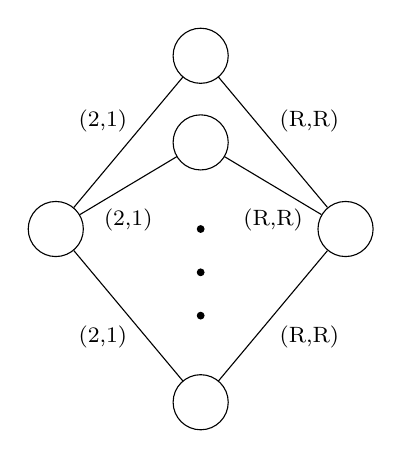
\begin{tikzpicture}[xscale=0.92,yscale=1.1]
      \tikzstyle{dot}=[circle,inner sep=1pt,fill=black];
      \tikzstyle{vtx}=[circle,draw,minimum size=7mm,fill=white];
      \tikzstyle{every node}=[font=\footnotesize];
      \node (s) at (-2,0) [vtx] {};
      \node (t) at (2,0) [vtx] {};
      \foreach \y in {-2, 1,2} {
        \draw (s) -- (0,\y) -- (t);
      }
      \foreach \y in {0,-0.5,-1} {
        \node at (0,\y) [dot] {};
      }
      \node at (0,2) [vtx] {};
      \node at (0,1) [vtx] {};
      \node at (0,-2) [vtx] {};
      \node at (-1.35,1.25) {(2,1)}; \node at (1.5,1.25) {(R,R)};
      \node at (-1.35,-1.25) {(2,1)}; \node at (1.5,-1.25) {(R,R)};
      \node at (-1,0.1) {(2,1)}; \node at (1,0.1) {(R,R)};
    \end{tikzpicture}
\end{boxedminipage}
}

\noindent There is an edge of capacity  and cost  (call these
\emph{small} edges) between  and each , and an edge of
capacity  and cost  between each  and  (\emph{large}
edges). We have . Clearly, an optimal integral solution
must select at least  of the large edges (in addition to small
edges), and hence has cost greater than .  The instance is
depicted in the accompanying figure: Label  on an edge denotes
capacity  and cost .




We now describe a feasible LP solution: set  on each small
edge , and  on each large edge . The cost of this
solution is  from the small edges, and  from the large edges,
for a total of . This is a factor of  smaller
than the optimal integral solution, proving the desired integrality
gap.

\medskip
It remains only to verify that this is indeed a feasible solution to
\KCLP. Consider the constraint corresponding to sets . As edges
in  play no role, we may assume . If  includes a large edge, or at least  small
edges, the residual requirement  that must be satisfied by the
remaining edges of  is , and so the constraint is
trivially satisfied. Let  consist of  small edges; the
residual requirement is thus . Let  contain  large
edges and thus  small edges. Now, the contribution to the left
side of the constraint from small edges in  is
. Therefore, the residual
requirement is satisfied by small edges alone unless .  But
the contribution of large edges is 
which is greater than  whenever . Thus, we satisfy each
of the added KC inequalities.

\subsection{Hardness of Approximation in Directed Graphs}
\label{subsec:stHardness}

We now prove Theorem \ref{thm:stHardness} via a reduction from the label
cover problem~\cite{ABSS}.

\begin{definition} [{\em Label Cover Problem}]
  The input consists of a bipartite graph  such that the degree
  of every vertex in  is  and degree of every vertex in  is
  ,  a set of labels  and a set of labels , and  a
  relation  for each
  edge .  Given a labeling ,
  an edge  is said to be {\em consistent} iff
  . The goal is to find a
  labeling that maximizes the fraction of consistent edges.
\end{definition}

The following hardness result for the label-cover problem is a well-known
consequence of the PCP theorem~\cite{ALMSS} and Raz's Parallel Repetition
theorem~\cite{Raz98}.

\begin{theorem}[{\rm \cite{ALMSS,Raz98}}]
\label{thm:labelcover_hard}
For any , there does not exist a poly-time algorithm
to decide if a given instance of label cover problem
has a labeling where all edges are consistent {\rm (\yes)}, or
if no labeling can make at least  fraction
of edges to be consistent for  {\rm (\no)},
unless .
\end{theorem}

We now give a reduction from label cover
to the single-pair Cap-SNDP in directed graphs. 
In our reduction, the only non-zero capacity values will be , , and . 
We note that Theorem~\ref{thm:labelcover_hard} holds even when we restrict 
to instances with . Thus our hardness result will hold on single-pair Cap-SNDP
instances where there are only two distinct non-zero capacity values.


Given an instance 
of the label cover problem with  edges, we create in polynomial-time a directed
instance  of single-pair Cap-SNDP such that if  is a \yes
then  has a solution of cost at most , and otherwise,
every solution to  has cost
. This establishes Theorem \ref{thm:stHardness}
when we choose .

The underlying graph  for the single-pair Cap-SNDP instance
is constructed as follows.  The set  contains a vertex  for every
. We slightly abuse notation and refer to
these sets of vertices in  as  and  as well.
Furthermore, for every vertex , and for every label , the set  contains a vertex . Similarly, for every vertex , and for every label , the set  contains a vertex
. Finally,  contains  a source vertex  and a sink vertex .
The set  contains the following directed edges:

 \vspace{-3mm}
\begin{itemize}
\item For each vertex  in , there is an edge from  to the
  vertex  of cost  and capacity . For each vertex
  , there is an edge from  to  of
  cost  and capacity .

\item For each vertex , and for all labels  in , there is
  an edge from  to  of cost  and
  capacity . For each vertex , and for all labels  in ,
  there is an edge from  to  of cost 
  and capacity . These two types of edges are the only edges
  with non-zero cost.

\item For every edge , and for every pair of labels
  , there is an edge from 
  to  of cost  and capacity .
\end{itemize}
\vspace{-2mm}
\noindent
This completes the description of the network . The requirement
 between  and  is , the number of edges in the label cover instance.
It is easy to verify that the size of the graph  is at most quadratic
in the size of the label cover
instance, and that  can be constructed in polynomial-time.
The lemmas below analyze the cost of \yes and \no instances.

\begin{lemma}\label{lemm:yes}
If the label cover instance is a \yes, then  contains a subgraph
of cost  which can realize a flow of value  from  to .
\end{lemma}
\begin{proof}Let  be any labeling that consistently labels all edges in .
Also, let  be the set of all edges of cost  in , and
let  be  the set of edges . We claim that  is a feasible
  solution for the single-pair Cap-SNDP instance.
  Note that the total cost of edges in  is .
  We now exhibit a flow of value  from  to  in .
   A flow of value  is sent along the path  for all .  From , a unit of flow is sent
  to the  vertices of the form ; this is feasible because   consistently
    labels all edges in .  Thus each vertex of the form 
    where  receives 
  units of flow, since the degree of  is  in .  A flow of
  value  is sent to  along the path . Thus 
  sends out a flow of value , or equivalently,  receives a flow of value
  .
\end{proof}

\begin{lemma}\label{lem:no}
If the label cover instance is a \no,
then any subgraph of  that realizes a flow of  units from  to 
has cost .
\end{lemma}
\begin{proof}
 Let , and .  Assume by way of
  contradiction, that there exists a subgraph  of  of
  cost strictly less than  that realizes  units
  of flow from  to . We say a vertex  is {\em light} if
  the number of edges of the form  in
   is less than . Similarly, we say a vertex  is
  {\em light} if the number of edges of the from
   in  is less than . All
  other vertices in  are referred to as {\em heavy}
  vertices. Note that at most  fraction of vertices in  could
  be heavy, for otherwise the total cost of the edges in  would
  exceed . Similarly, at most  fraction of vertices in  could
  be heavy.

  Now fix any integral - flow  of value  in ; an
  integral flow exists since all capacities are integers. We start by
  deleting from  all heavy vertices.  Since at most 
  fraction of either  or  are deleted, the total residual flow
  in this network is at least 
  (recall that ) since at most  units of flow can
  transit through a vertex in , and at most  units of flow can
  transit through a vertex in .

  Let  be a decomposition of the residual flow into unit flow
  paths.  Note that .  By construction of , every flow
  path  is of the form  where the pair
  .  We say that an edge  is a {\em good} edge if there is a flow path  of the above
  form, and we say  is a certificate for edge  being good.
  Note that every flow path  is a certificate of exactly one edge
  .  We claim that there are at least  good
  edges in .  It suffices to show that for any edge ,
  at most  flow paths in  can certify that  as a
  good edge.  Since  and  are both light vertices, we know that
   and . Now using the
  fact that each edge  has unit capacity, it follows
  that at most  paths in  can certify  as a good
  edge.  Hence number of good edges in  is at least
  .

  We now show existence of a labeling  that makes at least
   fraction of the edges to be consistent,
  contradicting that we were given a \no of label cover. For a vertex
  , let .  Similarly, we define  for each vertex .
  Consider the following random label assignment: each vertex  is assigned uniformly at random a label from , and
  each vertex in  is assigned uniformly at random a label in
  . For any good edge , the probability that the
  random labeling makes it consistent is at least 
  since  and  are both less than  (as
   and  are light), and there exists an 
  and  such that .  Thus, in expectation, at least 
  fraction of good edges are made consistent by the random assignment.
  Hence there exists a labeling  that  edges in  consistent.
  \end{proof}
Since the graph  can be constructed from  in poly-time,
it follows that a poly-time -approximation algorithm
for single-pair Cap-SNDP would give a poly-time algorithm to
decide whether a given instance of label cover is a \yes or a \no.

\section{Cap-SNDP with Multiple Copies Allowed} \label{sec:multipleCopies}

We now consider the version of Cap-SNDP when multiple copies of any
edge  can be chosen; that is, for any integer ,
 copies of  can be bought at a cost  to
obtain a capacity of .  Allowing multiple copies
makes the problem easier, and Goemans \etal \cite{GG+} give a  factor approximation algorithm for the problem.  In this
section, we complement this result with a  factor
approximation algorithm, where  is the number of  pairs with
.\footnote{Note that we overload the letter `',
  previously used in the definition of the \kway problem; this should
  cause no ambiguity as we discuss only pairwise connectivity
  requirements in this section.} Our algorithm is inspired by the work
of Berman and Coulston \cite{BC} on online Steiner Forest.  For
notational convenience, we rename the pairs , and denote the requirement  as ; the
vertices  are referred to as \emph{terminals}. We also
assume that the pairs are so ordered that .

We first give an intuitive overview of the algorithm. The algorithm
considers the pairs in decreasing order of requirements, and maintains
a \emph{forest solution} connecting the pairs that have been already
been processed; that is, if we retain a single copy of each edge in
the partial solution constructed so far, we obtain a forest . For
any edge  on the path in  between  and , the total
capacity of copies of  will be at least . When considering
, we connect them as cheaply as possible, assuming that
edges previously selected for  have  cost. (Note that this can
be done since we are processing the pairs in decreasing order of
requirements and for each edge already present in , the capacity of
its copies is at least .) The key step of the algorithm is that
\emph{in addition} to connecting  and , we also connect the
pair to certain other components of  that are ``nearby''.  The cost
of these additional connections can be bounded by the cost of the
direct connection costs between the pairs. These additional
connections are useful in allowing subsequent pairs of terminals to be
connected cheaply. In particular, they allow us to prove a 
upper bound on the approximation factor.

We now describe the algorithm in more detail. The algorithm maintains
a forest  of edges that have already been bought;  satisfies the
invariant that, after iteration , for each , 
contains a unique path between  and . In iteration , we
consider the pair .  We define the cost function  as
 for edges  already in , and , for edges . Note that for an edge
, the cost  is sufficient to buy enough copies of
 to achieve a total capacity of . Thus it suffices to connect
 and  and pay cost  for each edge; in the Cap-SNDP
solution we would pay at most this cost and get a feasible solution.
However, recall that our algorithm also connects  and  to 
other ``close'' components; to describe this process, we introduce
some notation:

For any vertices  and , we use  to denote the distance
between  and  according to the metric given by edge costs
. We let  be the cost required to
connect  and , given the current solution . We also
define the \emph{class} of a pair , and of a component:
\vspace{-2mm}
\begin{itemize}
  \item For each , we say that pair  is in
    \emph{class}  if .\\
    Equivalently, .

  \item For each connected component  of , . 
\end{itemize}

\vspace{-2mm}
\noindent 
Now, the algorithm connects  (respectively ) to component
 if  (resp.~) . That is, if  is close to the pair 
compared to the classes they are in, we connect  to the pair. As we
show in the analysis, this extra connection cost can be charged to
some pair  in the component . The complete algorithm
description is given below.


\iffalse 
We define the algorithm more precisely below.  At every stage of the
algorithm we maintain a forest  in which every pair seen so far is
connected.  In iteration We now divide the pairs into various classes
based on their connection costs.  In particular, we say a pair
 is in {\em class}  if .
Equivalently, . For a component 
in , we define . Depending on the classes of the various components in ,
we connect  to some additional components. In particular, if
either  or  is less
than , then we connect  or 
to .
\fi

\begin{algo}
  \underline{\sc Cap-SNDP-MC}:\\
   \hspace{2.26in}\Comment{ is the forest
    solution returned} \\
  For  to  \+ \\
    For each edge ,  \\
    For each edge ,  \\
     \\
    Add to  a shortest path (of length ) from  to
     under distances  \\
     \\
    For each connected component  of  \+ \\
      If  \+ \\
        Add to  a shortest path connecting  and  \- \- \\
    For each connected component  of  \+ \\
      If  \+ \\
        Add to  a shortest path connecting  and  \- \- \\       
    Buy  copies of each edge  added during this iteration. \-
\end{algo}
\iffalse
Note that though the forest  may change several times during a
single iteration  of the outer loop, the costs  are fixed
at the beginning of each iteration. Also, the components of  may
change during the final loops; thus, these loops run over the
components that have not been merged with the component containing
 and .
\fi
We prove that this algorithm {\sc Cap-SNDP-MC} gives an 
approximation. \\

\noindent
The structure of our proof is as follows: Recall that  was the
direct connection cost between  and ; in addition to paying
 to connect these vertices, the algorithm also buys additional
edges connecting  and  to existing components. We first show
(in Lemma~\ref{lem:ellPays}) that the total cost of extra edges bought
can be charged to the direct connection costs; thus, it suffices to
show that , where  is the cost
of an optimal solution.  To prove this (Lemma~\ref{lem:lowerBound}),
we bucket the pairs  into  groups based on
, and show that in each bucket , .

\iffalse
\begin{prop}
  {\sc Cap-SNDP-MC} returns a feasible solution.
\end{prop}
\begin{proof}
  {\bf Entirely trivial; included just for completeness. Might as well
    be removed.-- Nitish} We prove by induction on  that after
  iterations  through ,  contains a path between  and
   for each . Further, for each edge  added in
  iterations , the total capacity of the copies of 
  is at least .

  Consider any iteration ; as we only add edges to , the
  hypothesis is still satisfied for each pair  with . Since we add to  a shortest path between  and , 
  clearly contains the desired path. Consider any edge  on this
  path: If it was added in iteration , the total capacity of
  its copies is at least ; if it was added during
  iteration , the total capacity of its copies is
  . Thus, the capacity of (the
  copies of) any edge along the path from  to  is at least
  , giving a feasible solution.
\end{proof}
\fi

\begin{lemma}\label{lem:ellPays}
  The total cost of all edges bought by {\sc Cap-SNDP-MC} is at most
  .
\end{lemma}
\begin{proof}
  Let  denote the set of edges added to  during iteration
  . First, note the total cost paid for copies of edge 
  is . Thus, it suffices to show:
   

  We prove that the total cost of the \emph{additional} edges bought
  is at most ; this clearly implies the desired
  inequality. It is \emph{not} true that for each , the total cost
  of additional edges bought during iteration  is at most .  Nonetheless, a careful charging scheme proves the needed bound
  on total cost.  In iteration , suppose we connect the pair
   to the components . We charge the cost
  of connecting  and component  to the connection
  cost  of a pair  in . This is possible since
  we know the additional connection cost is at most
  . Care is required to ensure no pair is
  overcharged. To do so, we introduce some notation.


  At any point during the execution of the algorithm, for any current
  component  of , we let  be a pair  such that . For integers ,  will denote a pair  in ; we
  explain how this pair is chosen later. (Initially,  is
  undefined for each component .)

  Now, we have to account for additional edges bought during iteration
  ; these are edges on a shortest path connecting  (or )
  to some other component ; we assume w.l.o.g.~that the path is
  from  to . Consider any such path  connecting  to a
  component ; we have . Let : Charge all edges on this path to  if it is
  defined; otherwise, charge all edges on the path to . In
  either case, the pair () becomes the  of the new
  component just formed. Note that a pair  could
  simultaneously be the -, -, etc. for a
  component  if  connected to many components during
  iteration . However, it can never be the  of a
  component for , and once it has been charged as
  , it is never charged again as .  Also observe
  that if a pair is in a component  whose  is defined,
  subsequently, it always stays in a component in which the 
  is defined.

  \medskip
  For any , we claim that the total charge to pair  is
  at most , which completes the proof. Consider any such
  pair: any charges to the pair occur when it is either  or
   of its current component. First, consider charges to
   as  of a component. Such a charge can only
  occur when connecting some  (or ) to . Furthermore, if
  , the
   must be \emph{currently undefined}, for otherwise the
   would have been charged.  Subsequently, the 
  of the component containing  is always defined, and so
   will never again be charged as a  by a path
  of length in . Therefore, the total charge to  as  of a component is at most .

  Finally, consider charges to  as  of a
  component. As observed above, .  Also for a fixed
  , a pair is charged at most once as . Since the total
  cost charged to  as  is at most ;
  summing over all , the total charge is less than
  .

  Thus, the total charge to  is at most , completing the proof.
  \end{proof}

\begin{lemma}\label{lem:lowerBound}
  If  denotes the cost of an optimal solution to the instance of
  Cap-SNDP with multiple copies, then .
\end{lemma}
\begin{proof}
  Let  denote . Clearly,
  . 
  The lemma follows from the two sub-claims below:

  \noindent \textbf{Sub-Claim 1: }
  

  \noindent \textbf{Sub-Claim 2: }
  For each , .

  \begin{proofof}{Sub-Claim 1}
    Let . We have , and for
    any terminal  such that ,
    we have . Thus, the total
    contribution from such classes is at most , and hence:
    \vspace{-5mm}
    
  \end{proofof}


  \bigskip \def\ball{{\tt ball}}

  It remains to show Sub-Claim 2, that for each , .  Fix .  Let  denote the set of pairs  such
  that .  Our proof will go via the natural primal and
  dual relaxations for the Cap-SNDP problem. In particular, we will
  exhibit a solution to the dual relaxation of cost . To do so
  we will require the following claim.  Define , a {\em
    ball} of radius  around  as containing the set of vertices
   such that  and the set of edges  such
  that . An edge  is
  \emph{partially} within the ball if . Subsequently, we assume for ease of
  exposition that no edges are partially contained within the balls we
  consider; this can be achieved by subdividing the edges as
  necessary. Similarly, we define , the ball of radius
   around . Two balls are said to be \emph{disjoint} if they
  contain no common vertices.
  
  \begin{claim}\label{claim:balls}
    There exists a subset of pairs, , , and a collection of  disjoint balls of radius
     centred around either  or , for every pair
    .
  \end{claim}
  
  We prove this claim later; we now use it to complete the proof of
  Sub-Claim 2.  First we describe the LP.  Let the variable 
  denote whether or not edge  is in the Cap-SNDP solution. Let
   be the set of paths from  to . For each , variable  denotes how much flow  sends to the root
  along path . We use  to refer to , the
  effective capacity of edge  for pair .

  \begin{tabular}{c|l}
    \begin{minipage}[htb]{0.45\linewidth}
      
    \end{minipage}
    &
    \begin{minipage}[htb]{0.45\linewidth}
      
    \end{minipage}
  \end{tabular}


  We now describe a feasible dual solution of value at least 
  using Claim \ref{claim:balls}. 
For , if there is a ball  around  (or
  equivalently ), we define  for each
  edge in the ball. Since the balls are disjoint, the first inequality
  of the dual is clearly satisfied.  Set . For
  any path , we have
  

\noindent
  where the first inequality used , the second follows
  from the definition of , and the last inequality follows
  from the definition of . Thus,  is feasible along with these 's. This gives
  a total dual value of

  
  where the last inequality follows from the fact that . This proves the lemma modulo Claim \ref{claim:balls}, which we
  now prove.

  \begin{proofof}{Claim \ref{claim:balls}}
    We process the pairs in  in the order they are processed by
    the original algorithm and grow the balls.  We abuse notation and
    suppose these pairs are . We maintain
    a collection of disjoint balls of radius , initially
    empty.

    At stage , we try to grow a ball of radius  around either
     or . If this is not possible, the ball around 
    intersects that around some previous terminal in , say
    ; similarly, the ball around  intersects that of a
    previous terminal, say .  Let  be a vertex in
     and . We have . (The second inequality follows because for any  and
    any edge , .) Similarly, we have .

    Now, we observe that  and  could not have been in the
    same component of  at the beginning of iteration  of {\sc
      Cap-SNDP-MC}; otherwise , contradicting that . But
    since  and , we
    connect  to the component of  during iteration ;
    likewise, we connect  to the component of  during
    this iteration. Hence, at the end of the iteration,  are all in the same component. As a result, the
    number of components of  containing pairs of 
    \emph{decreases} by at least one during the iteration.

    It is now easy to complete the proof: During any iteration of 
    corresponding to a pair , the number of
    components of  containing pairs of  can go up by at most
    one. Say that an iteration \emph{succeeds} if we can grow a ball
    of radius  around either  or , and \emph{fails}
    otherwise.  During any iteration that fails, the number of
    components decreases by at least one; as the number of components
    is always non-negative, the number of iterations which fail is no
    more than the number which succeed. That is, .
  \end{proofof}
\end{proof}

Theorem~\ref{thm:multipleCopies} is now a straightforward consequence
of Lemmas~\ref{lem:ellPays} and \ref{lem:lowerBound}:

\begin{proofof}{Theorem~\ref{thm:multipleCopies}}
  The total cost of edges bought by the algorithm is at most
  , by
  Lemma~\ref{lem:ellPays}. But , by Lemma~\ref{lem:lowerBound}, and hence the total
  cost paid by {\sc Cap-SNDP-MC} is at most . 
\end{proofof}




\section{Conclusions} \label{sec:conclusions} 

In this paper we made progress on addressing the approximability of
Cap-SNDP. We gave an  approximation for the \capR problem,
which is a capacitated generalization of the well-studied min-cost
-edge-connected subgraph problem. Can we improve this to obtain an
 approximation or prove super-constant factor hardness of
approximation? We also highlighted the difficulty of Cap-SNDP by
focusing on the single pair problem, and showing both super-constant
hardness and an  integrality gap example, even for the LP
with KC inequalities. We believe that understanding the single pair
problem is the key to understanding the general case. In particular,
we do not have a non-trivial algorithm even for instances in which the
edge capacities are either  or ; this appears to capture much of
the difficulty of the general problem. As we noted, allowing multiple
copies of edges makes the problem easier; in practice, however, it may
be desirable to not allow too many copies of an edge to be used. It is
therefore of interest to examine the approximability of Cap-SNDP if we
allow only a small number of copies of an edge. Does the problem admit
a non-trivial approximation if we allow  copies or, say,  copies? This investigation may further serve to delineate the easy
versus difficult cases of Cap-SNDP.

\paragraph{Acknowledgements:} CC's interest in capacitated network
design was inspired by questions from Matthew Andrews. He thanks
Mathew Andrews and Lisa Zhang for several useful discussions
on their work on capacitated network design for multi-commodity
flows.

\begin{thebibliography}{10}
\bibitem{And} M. Andrews.  \newblock Hardness of Buy-at-Bulk Network
  Design.  \newblock In {\em Proceedings, IEEE Foundations of Computer
    Science (FOCS)}, pp 115--124, 2004.

\bibitem{AZ} M. Andrews and L. Zhang. Personal Communication, 2009.

\bibitem{ALMSS}
S.~Arora, C.~Lund, R.~Motwani, M.~Sudan, and M.~Szegedy.
\newblock Proof verification and the hardness of approximation problems.
\newblock {\em Journal of the ACM}, 45(3):501--555, 1998.

\bibitem{ABSS}
S. Arora, L. Babai, J. Stern, and Z. Sweedyk.
\newblock The Hardness of Approximate Optimia in Lattices, Codes, and Systems of Linear Equations.
\newblock {\em J. Comp. Sys. Sci.} 54(2):317--331, 1997.



\bibitem{BC}
P. Berman and C. Coulston.
\newblock On-Line Algorithms for Steiner Tree Problems (Extended Abstract). 
\newblock In {\em Proceedings, ACM Symposium on Theory of Computation (STOC)}, pp. 344--353, 1997.

\bibitem{CFLP}
R.~D. Carr, L.~K. Fleischer, V.~J. Leung, and C.~A. Phillips.
\newblock Strengthening integrality gaps for capacitated network design and
  covering problems.
\newblock In {\em Proceedings, ACM-SIAM Symposium on Discrete Algorithms (SODA)},
  pp. 106--115, 2000.



\bibitem{CNS}
M. Charikar, J. Naor, and B. Schieber.
\newblock Resource optimization in QoS multicast routing of real-time multimedia.
\newblock {\em IEEE/ACM Trans. Netw. }12(2):340--348, 2004.



\bibitem{CHKS}
C.Chekuri, M. T. Hajiaghayi, G. Kortsarz, and M. R. Salavatipour.
\newblock Approximation Algorithms for Non-Uniform Buy-at-Bulk Network Design.
\newblock In {\em Proceedings, IEEE Symposium on Foundations of Computer Science (FOCS)}, pp. 677--686, 2006.

\bibitem{CGNS}
J. Chuzhoy, A. Gupta, J. Naor and A. Sinha.
\newblock On the approximability of some network design problems.
\newblock {\em ACM Transactions on Algorithms}, 4(2), 2008.

\bibitem{ChuzhoyK08}
J.~Chuzhoy and S.~Khanna.
\newblock {Algorithms for single-source vertex connectivity}.
\newblock In {\em Proceedings of the 49th Annual IEEE Symposium on Foundations
  of Computer Science}, pages 105--114, 2008.

\bibitem{CKsndp}
J.~Chuzhoy and S.~Khanna.
\newblock {An -Approximation Algorithm for Vertex-Connectivity
  Survivable Network Design}.
\newblock In {\em Proceedings of the 50th Annual IEEE Symposium on Foundations
  of Computer Science}, pages 437--441. IEEE, 2009.






\bibitem{Fer}
C. G. Fernandes.
\newblock A better approximation ratio for the minimum k-edge-connected spanning subgraph problem.
\newblock In {\em Proceedings, ACM-SIAM Symposium on Discrete
  Algorithms (SODA)}, pp. 629--638, 1997.

\bibitem{FleischerJW}
L.~Fleischer, K.~Jain, and D.P. Williamson.
\newblock {Iterative rounding 2-approximation algorithms for minimum-cost
  vertex connectivity problems}.
\newblock {\em Journal of Computer and System Sciences}, 72(5):838--867, 2006.

\bibitem{GG+}
M. X. Goemans, A. V. Goldberg, S. A. Plotkin, D. B. Shmoys, \'{E}. Tardos, and D. P. Williamson.
\newblock Improved Approximation Algorithms for Network Design Problems
\newblock In {\em Proceedings, ACM-SIAM Symposium on Discrete Algorithms (SODA)},
  pp. 223--232, 1994.









\bibitem{Jain}
K. Jain.
\newblock A Factor 2 Approximation Algorithm for the Generalized Steiner Network Problem
\newblock {\em Combinatorica}, 21(1): 39--60, 2001.

\bibitem{Karger}
David Karger.
\newblock Random Sampling in Graph Optimization Problems.
\newblock Ph.D. Thesis, Stanford University, 1994.

\bibitem{KortsarzN}
G.~Kortsarz and Z.~Nutov.
\newblock {Approximating minimum cost connectivity problems}.
\newblock In T.F. Gonzalez, editor, {\em Handbook of Approximation algorithms
  and Metaheuristics}. CRC Press, 2007.







\bibitem{MR}
R. Motwani, and P. Raghavan.
\newblock Randomized Algorithms.
\newblock {\em Cambridge University Press}, 1995.

\bibitem{NutovBifamiliesFOCS}
Z.~Nutov.
\newblock {Approximating minimum cost connectivity problems via uncrossable
  bifamilies and spider-cover decompositions}.
\newblock In {\em Proceedings of the fiftieth Annual IEEE Symposium on
  Foundations of Computer Science}, pages 417--426. IEEE, 2009.



\bibitem{Raz98}
R.~Raz.
\newblock A parallel repetition theorem.
\newblock {\em SIAM Journal of Computing}, 27(3):763--803, 1998.










\end{thebibliography}

\appendix

\section{Hardness of Approximation for  Cap-SNDP in Undirected Graphs}
\label{app:copiesHardness} 


In this section, we prove Theorem~\ref{thm:copiesHardness} via a
reduction from the \emph{Priority Steiner Tree} problem. In the
Priority Steiner Tree problem, the input is an undirected graph
 with a cost  and a priority 
for each edge . (We assume  is the highest and  the lowest
priority.) We are also given a root  and a set of terminals ; each terminal  has a desired priority
. The goal is to find a minimum-cost Steiner Tree in which the
unique path from each terminal  to the root consists only of edges
of priority  or higher.\footnote{It is easy to see that a
minimum-cost subgraph containing such a path for each terminal is a
tree; given any cycle, one can remove the edge of lowest priority.}

Chuzhoy \etal \cite{CGNS} showed that one cannot approximate the
Priority Steiner Tree problem within a factor better than  unless , even when
all edge costs are  or . Here, we show an
approximation-preserving reduction from this problem to Cap-SNDP with
multiple copies; this also applies to the basic Cap-SNDP problem, as
the copies of edges do not play a significant role in the
reduction. 

Given an instance  of Priority Steiner Tree on graph
 with edge costs in , we construct an instance
 of Cap-SNDP defined on the graph  as the
underlying graph.  Fix  to be any integer greater than  where
 is the number of edges in the graph .  We now assign a capacity
of  to each edge  with priority  in
. Each edge  of cost  in 
has cost  in , and each edge  of cost
 in  has cost  in
. Finally, for each terminal , set 
if ; for every other pair of vertices , .

Let  denotes the cost of an optimal solution to ;
note that ; we now argue that  has an
optimal solution of cost  iff  has an optimal
solution of of cost between  and . Given
a solution  to  of cost , simply select the
same edges for ; the cost in  is
at most  since in , we pay  for each
edge in  that has cost  in .  This is
clearly a feasible solution to  as each terminal 
has a path to  in  containing only edges with priority at
least , which is equivalent to having capacity at least
. Conversely, given a solution  to  with
cost in , select a single copy of each edge in 
as a solution to ; clearly the total cost is at most
. To see that this is a feasible solution, suppose that  did
not contain a path from some terminal  to the root  using edges
of priority  or more. Then there must be a cut separating 
from  in which all edges of  have capacity at most . But since  supports a flow of  from  to ,
it must use at least  edges (counting with multiplicity); this
implies that the cost of  is at least , a
contradiction.

\bigskip
We remark that a similar reduction also proves 
hardness for the single-pair Cap-SNDP problem without multiple copies:
One can effectively encode an instance of the single-source
Fixed-Charge Network Flow (FCNF, \cite{CGNS}), very similar to
single-source Cap-SNDP with multiple copies, as an instance of
single-pair Cap-SNDP \emph{without} multiple copies: Create a new sink
, and connect  to each original terminal  with a single
edge of cost  and capacity . The only way to send flow
 flow from  to the source  is for each
terminal  to send  to . Thus,
Theorem~\ref{thm:singlePairHardness} is a simple consequence of the
 hardness for single-source FCNF \cite{CGNS}.




\section{Omitted Proofs}
\label{app:omittedProofs}

\subsection{Proof of Theorem \ref{thm:uniform}: Near Uniform Cap-SNDP}
\label{app:nearlyUniform}

The algorithm described in Section \ref{sec:uniformReq} can be
extended to the case where requirements are \emph{nearly} uniform,
that is, if  for all pairs . We obtain an -approximation, while
increasing the running time by a factor of . We work
with a similar LP relaxation; for each set , we use
 to denote the
requirement of . Now, the original constraints are of the form

for each set , and we define the residual requirement for a set as
. The KC inequalities use
this new definition of .

Given a fractional solution  to the KC LP, we modify the
definitions of highly fractional and nearly integral edges: An edge
 is said to be nearly integral if , and highly fractional otherwise. Again, for a fractional
solution , we let  denote the set of nearly integral edges;
the set  of small cuts is now . From the cut-counting theorem, .  We use  to denote the set of \emph{large}
cuts, the sets .

As before, a fractional solution  is \emph{good} if the original
constraints are satisfied, and the KC Inequalities are satisfied for
the set of edges  and the sets in . These constraints can be
checked in time , so following the proof
of Lemma~\ref{lem:ell}, for constant , we can find a good
fractional solution in polynomial time.

The rounding and analysis proceed precisely as before: For each highly
fractional edge , we select it for the final solution with
probability . The expected cost of this
solution is at most  times that of the optimal
integral solution, and analogously to the proofs of
Lemmas~\ref{lem:largeCuts} and \ref{lem:smallCuts}, one can show that
the solution satisfies all cuts with high probability. This completes
the proof of Theorem \ref{thm:uniform}.



\subsection{Proof of Theorem~\ref{thm:kWay}}

To prove Theorem~\ref{thm:kWay}, we work with the generalization of
\KCLP given below. For any -way cut  and for any set of edges
, we use  to be .\footnote{For ease of notation, we assume that for any edge ,
  . This is not without loss of generality, but the
  proof can be trivially generalized: In the constraint for each
  -way cut  such that , simply use the
  minimum of  and .}

\vspace{-5mm}


As before, given a fractional solution  to this LP, we define 
(the set of nearly integral edges) to be . Define  to be the
fractional capacity on the edges.  Let i+1.  The solution  is
said to be {\em good} if it satisfies the following three conditions:

\begin{enumerate}
\item[(a)] If the capacity of  is , the capacity of any
  -way cut in  is at least ; equivalently  satisfies the
  original constraints.
\item[(b)] The KC inequalities are satisfied for the set  and the
  sets in , for each . Note that if (a) is
  satisfied, then by Lemma~\ref{lem:kWayCutCounting}, .
\item[(c)]  is at most the value of the optimum
  solution to the linear program (-way KC LP).
\end{enumerate}

Following the proof of Lemma~\ref{lem:ell}, it is straightforward to
verify that there is a randomized algorithm that computes a good
fractional solution with high probability in  time.

Once we have a good fractional solution, our algorithm is to select
, the set of nearly integral edges, and to select each highly
fractional edge  with probability . If  denotes the highly fractional edges that were
selected, we return the solution . As before, it is
trivial to see that the expected cost of this solution is  times that of the optimal integral solution. 

We show below that for any , we satisfy all -way cuts
with high probability; taking the union bound over the  choices
of  yields the theorem. 

As in Lemmas~\ref{lem:largeCuts} and \ref{lem:smallCuts}, we
separately consider the ``large'' and ``small'' -way cuts.
First, consider any small cut  in . From the Chernoff bound
(Lemma~\ref{lem:Chernoff}) and the KC inequality for  and ,
it follows that the probability we fail to satisfy  is at most
. From the cut-counting Lemma~\ref{lem:kWayCutCounting},
there are at most  such small cuts, so we satisfy all
the small  way cuts with probability at least
.

For the large -way cuts , we separately consider cuts of
differing capacities. For each , let  denote the
-way cuts  such that . Consider any cut ; if , then the cut  is clearly satisfied. Otherwise,
. But since we selected
each edge  in  for  with probability
, the Chernoff bound implies that we do not
satisfy  with probability at most .  The
cut-counting Lemma~\ref{lem:kWayCutCounting} implies there are most
 such cuts, so we fail to satisfy any cut
in  with probability at most . Taking the union
bound over all , the failure probability is at most .



\end{document}
